%************************************************
\chapter[Un modèle morphologique]{Un modèle morphologique de scènes sonores environnementales}\label{ch:psycho_model} 
%************************************************

\section{Motivations}

\subsection{Analyse sensorielle}
\label{sec:ch4_anaSo}

Comme nous l'avons vu à la section~\ref{sec:ch3_appCatDim}, l'étude expérimentale des paysages sonores adopte deux approches:

\begin{itemize}
\item l'approche catégorielle: la mise en évidence des catégories d'environnements ou sources sonores;
\item l'approche dimensionnelle: l'identification des dimensions perceptives engagées dans les processus cognitifs, et des indicateurs dont elles dépendent.
\end{itemize}

Ces approches s'inscrivent dans des démarches différentes:

\begin{itemize}
\item l'approche catégorielle veut identifier les objets d'intérêt  de l'environnement sonore;
\item l'approche dimensionnelle veut identifier les éléments caractérisant les qualités affectives perçues d'une scène.
\end{itemize}

Si l'on interroge les influences qu'ont les différents éléments constituant une scène sur les qualités affectives perçues, alors les deux approches se rejoignent naturellement. L'approche catégorielle permet d'établir la liste des éléments d'intérêt, laquelle liste peut servir de base à une annotation des stimuli utilisés par l'approche dimensionnelle afin d'étudier les contributions spécifiques de leurs éléments respectifs.

Nous pensons que la simulation offre un cadre expérimental élégant permettant de faire le lien entre les deux approches \gl{TODO: plus insister ?}.

D'une part, comme illustré à la figure~\ref{fig:paradigmeSimu1}, la simulation peut être vue comme l'approche inverse des épreuves catégorielles (\cf~Section~\ref{sec:ch3_appCategorielle}). Quand les épreuves catégorielles discrétisent l'environnement sonore sur la base d'un tri et/ou d'une description verbale réalisés  par un sujet, la simulation, elle, recompose cet environnement, à partir d'une banque imposée de sons isolés. Ainsi, les catégories sonores, point de sortie des épreuves catégorielles, constituent-elles la banque de sons, point d'entrée de la simulation.

D'autre part, la finalité de la simulation est de produire un environnement complet, dont la partition (\cf~Section~\ref{sec:ch4_modelDes}), \ie~ses caractéristiques structurelles et compositionnelles, est parfaitement connue. Les stimuli ainsi produits peuvent être utilisés par l'approche dimensionnelle, afin d'étudier de manière fine les contributions des différents éléments.

La simulation se pose donc comme un outil intermédiaire, faisant le lien entre les connaissances issues des études adoptant l'approche catégorielle, et les stimuli requis par l'approche dimensionnelle.

La simulation présente d'autres intérêts:

\begin{itemize}
\item \emph{intérêt pratique}: afin d'étudier l'importance relative des différentes sources, il est indispensable de disposer de stimuli dont la partition est connue. Une première solution, adoptée par \citep{lavandier2006contribution}, a été d'annoter les stimuli. L'annotation cependant est une solution limitée: 
\begin{enumerate}
\item l'opération est fastidieuse, longue, et difficile à mettre en œuvre sur de grandes banques de données;
\item connaître la position des différentes sources dans une mixture sonore ne permet pas d'isoler leurs caractéristiques physiques respectives, et donc de calculer des indicateurs acoustiques dédiés. En traitement du signal, la séparation des sources reste un problème ouvert\gl{TODO: citation}.
\end{enumerate}

Par la simulation, nous obtenons directement le stimuli et son annotation. Qui plus est, celle-ci est produite par le sujet lui-même, et non par un tiers. \gl{Par ailleurs, le fait de posséder les sons isolés permet de facilement calculer des indicateurs acoustiques spécifiques à chaque source sonore.}

\item \emph{intérêt écologique}: la validité écologique des stimuli est un problème fondamental en analyse sensorielle. Dans le cas de l'analyse des qualités affectives perçues, où l'on demande au sujet ``\,que pensez vous de la qualité $Q$ de cet environnement\,'', il s'agit de garantir que les stimuli proposés fassent sens par rapport à la représentation mentale que le sujet se fait: 

\begin{itemize}
\item  du monde sonore; 
\item  de la qualité $Q$. 
\end{itemize}

Il est possible, dans les approches classiques, de résoudre ces problèmes en étudiant de manière préalable les stimuli à enregistrer (\cf~Section~\ref{sec:ch3_ecologique}). 

La simulation, en renversant la question posée (``\,générer un environnement qui correspond à une certaine valeur de $Q$\,''), garantit la validité écologique des stimuli, par définition connectés à la représentation sonore du sujet, \gl{à condition que la banque de données et l'outil de simulation soient suffisamment expressifs}.

\item \emph{représentativité des stimuli}: toute étude sensorielle, qu'elle soit \emph{in situ} ou en laboratoire, doit sélectionner un nombre restreint d'environnements sonores à évaluer. Il s'agit, tant que faire se peut, de garantir que le substrat de stimuli proposé soit représentatif de l'ensemble des environnements étudiés, un déséquilibre dans l'élaboration dudit substrat pouvant affecter, \emph{in fine}, l'évaluation des stimuli. 

Dans le cas des études sur la perception des environnements urbains, il est d'usage d'isoler des zones d’intérêts (parc, rue, place, \cf~Section~\ref{sec:ch3_ecologique}), et de répartir équitablement les stimuli parmi ces zones. \gl{Cependant, l'environnement d'une même zone est changeant, aussi bien si l'on considère le type de source présent, que si l'on considère la structure des patterns temporels émis par ces sources (\eg~pour une même rue passante, un son de trafic sera plus dense, composé de plus d'événements de voiture à la fin des horaires de travail). Il est donc nécessaire de contrôler la diversité des sources qui y occurrent ainsi que la diversité structurelle de leurs séquences d'émission}, d'autant plus si l'on cherche à étudier l'influence spécifique des différentes sources. Cette étape est complexe.

Si la structure interne des paysages sonores est variable, la diversité des sources sonores qui les composent est plus contrôlable. Des environnements sonores de parcs et de rues peuvent comprendre des voix humaines, des bruits de pas, des sons de voitures etc. Seules les caractéristiques physiques, ainsi que les patterns d'occurrences de ces sources, vont varier. Évaluer des scènes simulées, à partir d'une banque de sons isolés (sources sonores), peut constituer une solution au problème de la diversité des stimuli. Considérons l'étude de l'agrément sonore dans l'environnement urbain. Dans un premier temps, les stimuli sont obtenus via une épreuve de simulation. Dans cette simulation, seule la qualité affective des stimuli est fixée (agréable/désagréable). Les sujets construisent alors les scènes directement en fonction de l'image qu'ils se font d'un environnement urbain agréable/désagréable, adaptant ainsi la structure de la scène à la qualité de l'environnement. Dans un deuxième temps, les scènes ainsi élaborées peuvent constituer des stimuli pour une analyse sémantique différentielle de l'agrément. Cette approche est celle utilisée dans nos travaux (\cf~Chapitre~\ref{ch:psycho_xp}). 

Enfin, la plupart des environnements que nous percevons sont relativement neutres, et ne provoquent pas en nous de réactions particulières. Il peut n'être pas évident d'évaluer des dimensions perceptives comme l'agrément, la gêne ou le confort, de ces environnements. Des scènes simulées, sur la base d'une qualité affective imposée (\eg~agréable), proposent, quant à elles, des versions stéréotypées des environnements ainsi qualifiés. On peut voir dans ces scènes un ``\,résumé cognitif\,'', riche et condensé des environnements étudiés. Isoler les éléments d'intérêt de ces scènes peut s'avérer plus facile.

\end{itemize}

\begin{figure}[t]
        \myfloatalign
        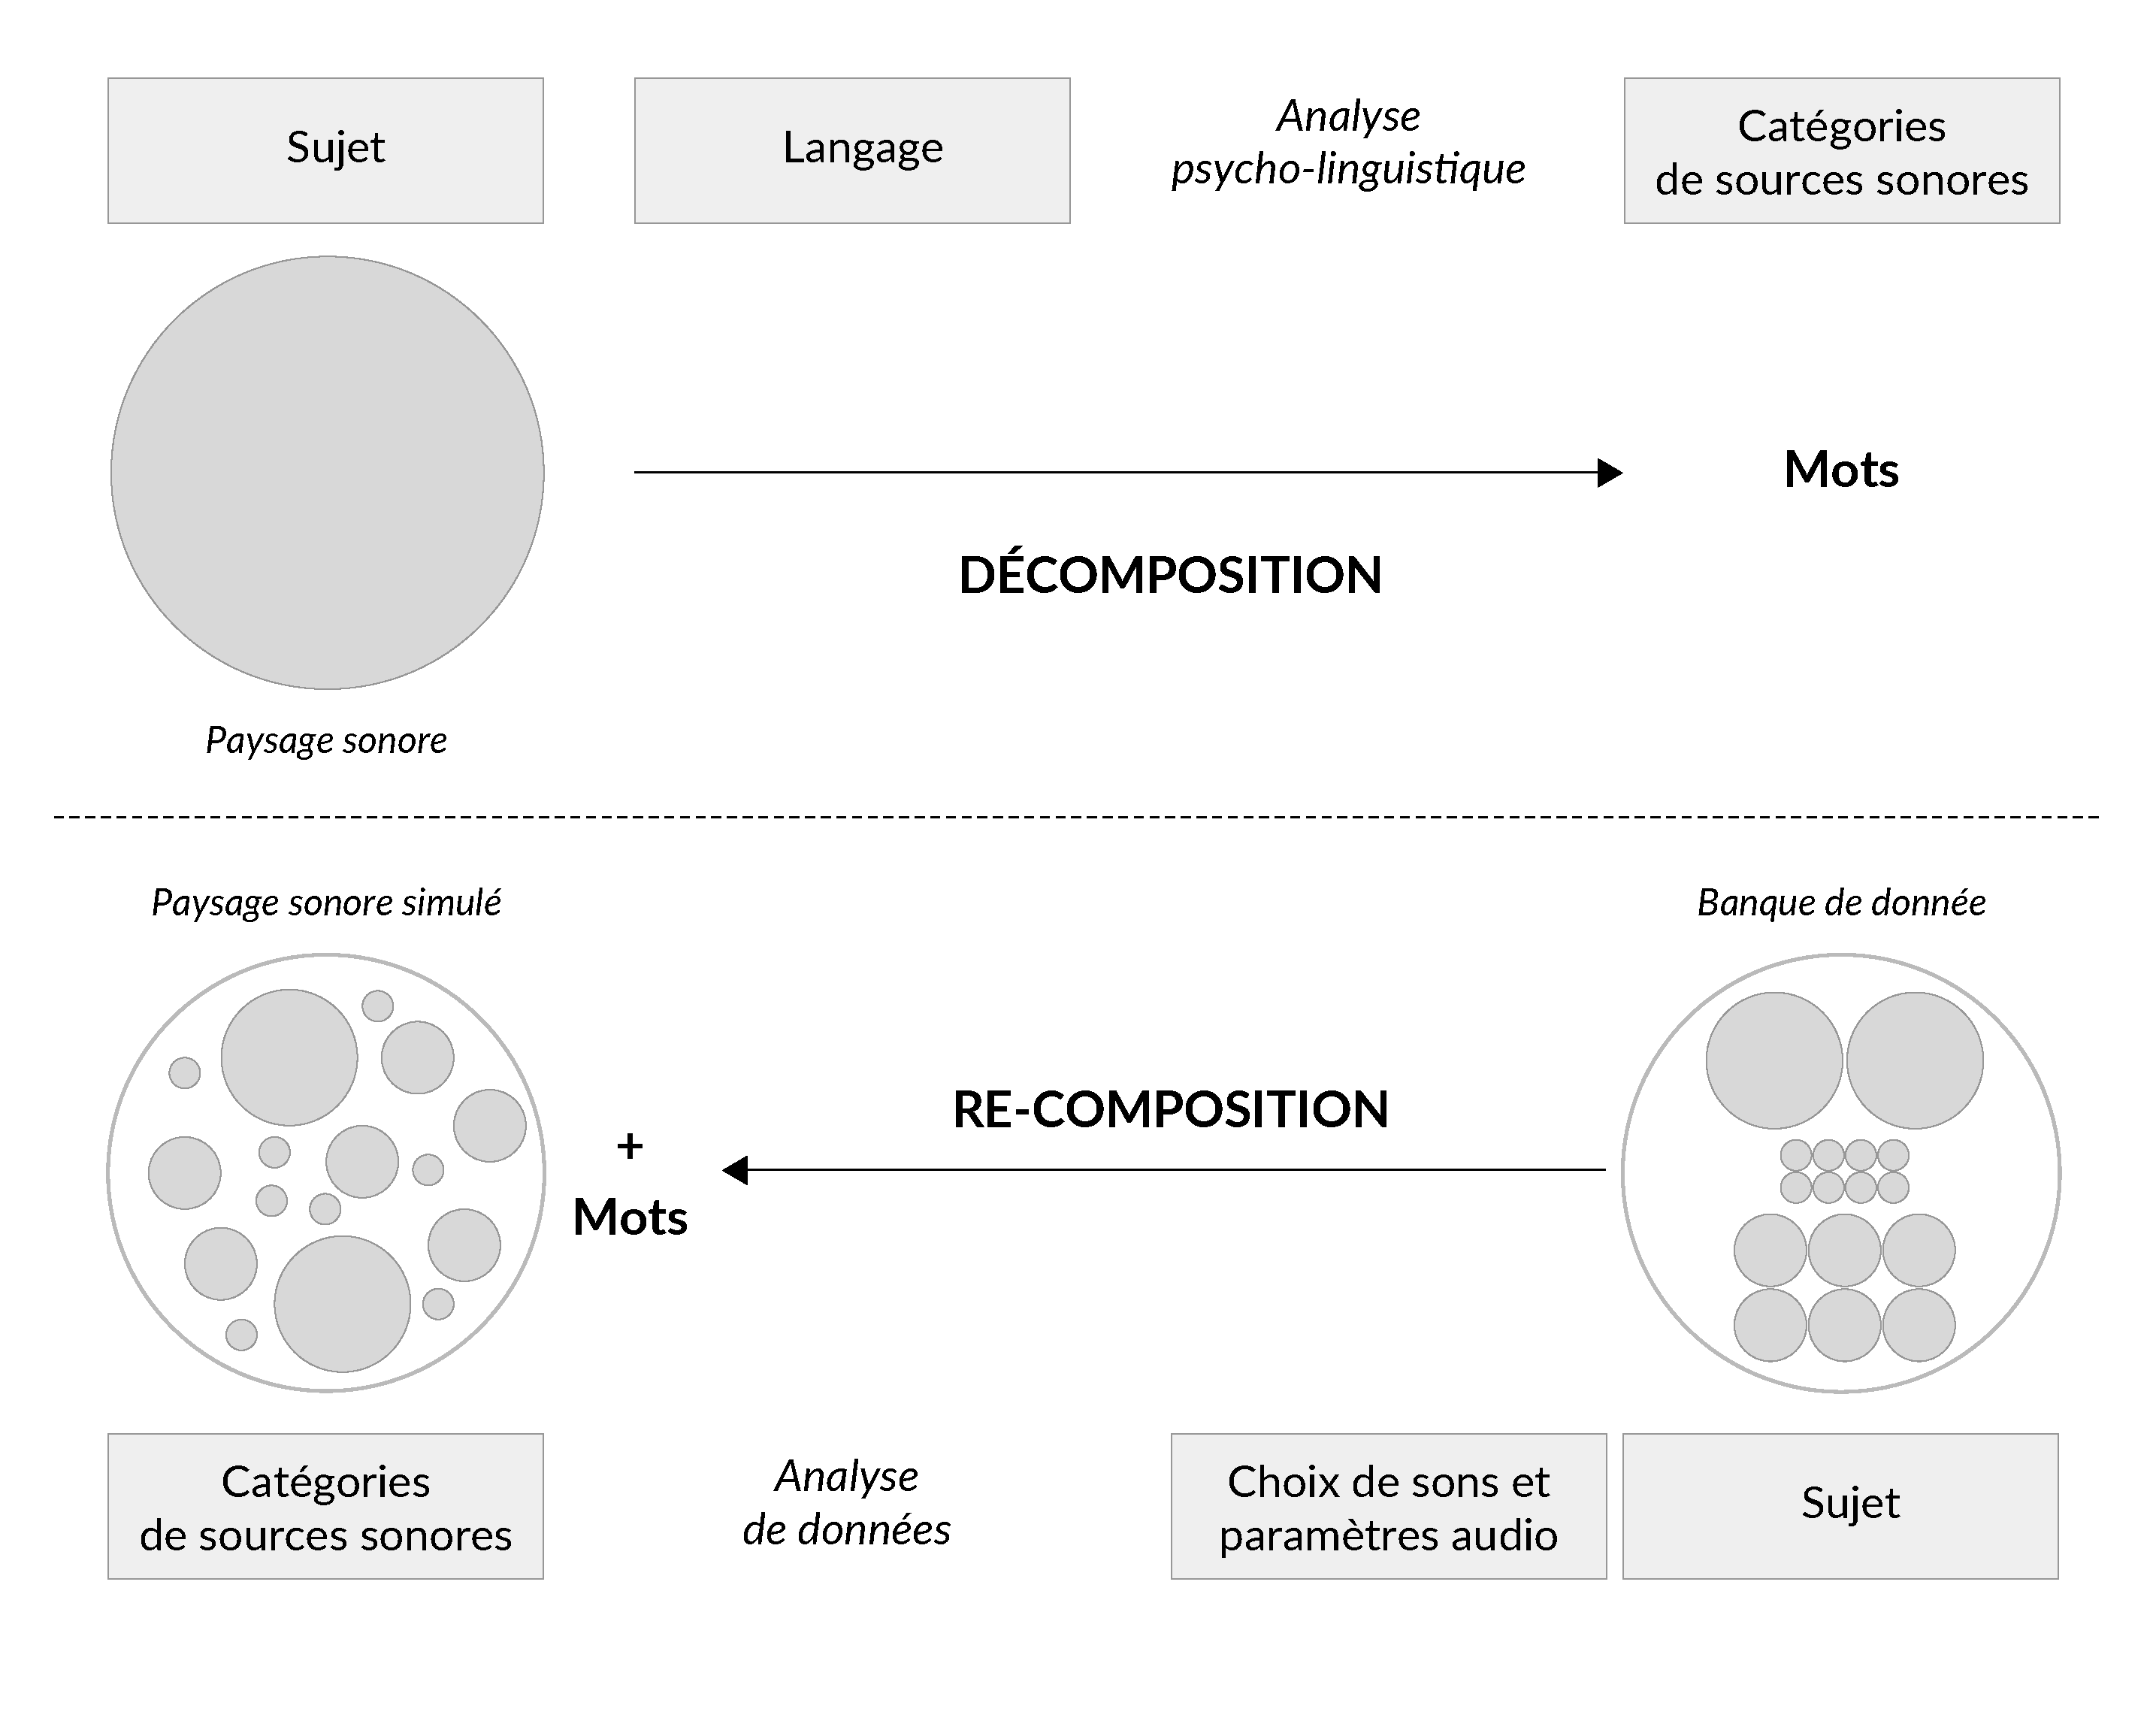
\includegraphics[width=.8\linewidth]{gfx/ch_4/1}
       \caption{TODO}\label{fig:paradigmeSimu1}
\end{figure}

\subsection{Analyse automatique}

\section{Proposition d'un modèle de scènes sonores}
\label{sec:ch4_model}

\subsection{Discrétiser l'environnement sonore}
\label{sec:ch4_modelInspi}


\subsubsection{L'unité de bases: la source sonore}

Les études portant sur l'ASA, et plus spécifiquement sur les processus de ségrégation, montrent, d'une part, que l'humain fait sens de son environnement en isolant les informations relatives aux différentes sources qui le composent, d'autre part, que ce groupement intervient très tôt dans la chaîne de traitement, et se base sur des règles génériques innées.\\

\gl{TODO: Neuroscience} \\ 

Dans le même temps, la recherche sur les paysages sonores, adoptant l’approche catégorielle, met en évidence que les processus de catégorisation s'appuient également sur la composition sémantique des scènes, \ie~les sources sonores identifiées. 

Pour notre modèle, il apparaît fondé de considérer comme élément de base la source sonore. Comme vu précédemment (\cf~Section~\ref{sec:ch3_categoEtAbstract}), la notion de source sonore est variable, un même objet pouvant être reconnu suivant plusieurs degrés d'abstraction.

\subsubsection{Typologie: niveaux d'abstractions et nomenclature source-action}
\label{sec:ch4_sourceAction}

La constitution de banques de sons peuplant l'environnement urbain est incontournable. Avant d'acquérir ces sources, \ie~de les enregistrer, il est nécessaire de les identifier. Une démarche naïve consisterait alors à établir la liste exhaustive de toutes les classes de sources sonores composant l'environnement. Une telle approche soulèverait deux problèmes:

\begin{itemize}
\item une source sonore peut se décrire en fonction de plusieurs niveaux d'abstraction. Identifier et nommer sont des actions déterminées par notre représentation mentale du monde (\cf~Section~\ref{sec:ch3_representationMentale}). Cette représentation s'organise, entre autre, suivant l'axe vertical des niveaux d'abstraction sur lequel s'appuie notre travail de catégorisation. Ainsi, si deux individus entendent un même son de voiture, il est possible que le premier le nomme ``\,voiture\,'' et le deuxième ``\,moteur\,''. Le dénombrement de l'ensemble des sources pouvant être utilisées par le modèle doit prendre en compte ce fait. Ces sources doivent être regroupées en classes hiérarchisées, afin de bâtir une structure taxonomique;
\item il n'existe pas de taxonomie standardisée des sources sonores. C'est une tradition des sciences modernes de classer et nommer les éléments avant de les étudier. Dans les domaines de la faune ou de la flore, une observation longue et minutieuse des sujets d'étude a permis d'élaborer un système de classification (taxonomie), et ainsi d'organiser et trier les objets en fonction de leurs propriétés partagées. Elle a permis encore d'élaborer une terminologie précise des classes d'objets. Grâce à quoi, la Biologie est devenue une science, laquelle science, au passage, devait donner naissance à la théorie de l'évolution \citep{lecointre2006tree}. Dans le domaine du son (ainsi que dans celui des odeurs), en revanche, point de système de classification \citep{dubois2000categories,niessen2010categories}. Nous trouvons à cela deux explications:

\begin{itemize}
\item \emph{champ lexical limité}: l'identification et la description d'un son sont des processus subjectifs étroitement liés au langage (\cf~Section~\ref{sec:ch3_catLang}). Deux sujets appartenant à deux groupes sociaux différents n'utiliseront pas les mêmes mots pour décrire un même objet. Pour établir un système de classification, il faut prendre une décision quant à la définition des termes utilisés. Or, contrairement au domaine de la vision, où une terminologie de base pour décrire les objets (couleur, forme etc.) est globalement partagée, le champ lexical applicable aux phénomènes acoustiques est, d'une part, limité (durée, fréquence...) \citep{dubois2000categories}, d'autre part, emprunté, dans une large mesure, à d'autres domaines perceptifs. On parle ainsi de brillance, ou de rugosité de sons. La diversité des termes descriptifs, et l'absence de consensus sur ce qu'ils désignent, rend difficile l'élaboration d'une classification standardisée;
\item \emph{influence du contexte}: L'identification et la description d'un son, section~\ref{sec:ch3_identification et Contexte} sont dépendantes du contexte, \ie~de la nature des sources cooccurrentes dans la scène \citep{ballas1987interpreting,niessen2008disambiguating,gygi2011incongruency}.
\end{itemize}
\end{itemize}

Il apparaît clairement que les classes de sons peuplant notre environnement doivent être organisées autour d'une taxonomie: un système de classes hiérarchisées. Cependant il y a un choix à faire quant à la manière de regrouper les sons à l'intérieur de cette taxonomie.

Comme vu à la section~\ref{sec:ch3_catSourceSoundScape}, plusieurs études ont montré que la catégorisation des sources sonores s'opère suivant des attributs sémantiques. Parmi ceux-ci, deux reviennent souvent:

\begin{itemize}
\item la source (agent, objet, fonction), \ie~l'objet émettant le son;
\item l'action, \ie~le mouvement physique à l'origine du son.
\end{itemize} 

Ces deux attributs fonctionnent de pair. S'inspirant de l'organisation catégorielle verticale à trois niveaux de Rosch (\cf~Section~\ref{sec:ch3_categoEtAbstract}), Guyot et al. \citep{guyot1997} proposent un système de catégorisation où les auditeurs identifient des groupements de sources abstraits, au niveau superordonné (``\,Bruit généré par une excitation mécanique\,''), des actions, au niveau de base (``\,gratter\,'',``\,frotter\,'') et des sources, au niveau subordonné (``\,vaisselle\,'',``\,stylo\,''). Reprenant à son tour ce système, \citep{houix_lexical_2012} montre que les sons sont catégorisés, en premier lieu, à partir du type de sources, et ensuite, seulement, à partir d'actions.

L'association source-action semble être une base sensée sur laquelle bâtir une taxonomie, dans laquelle les classes haut-niveaux sont des classes abstraites de sources sonores (``\,véhicule\,''), les classes intermédiaires, des classes de sources sonores (``\,voiture\,''), et les classes basses, des actions sonores (``\,passage\,''). Pour les classes de bas niveau, la perméabilité intra-classe est minimale.

Cette association source-action n'est cependant pas suffisante. Le choix des labels utilisés doit faire l'objet d'une sélection particulière. Ces labels doivent être génériques, compréhensibles, et décrire de manière non ambiguë les objets de la classe considérée. Afin de les choisir, il est possible de se référer aux travaux de Gaver \citep{gaver1993world}, qui propose une taxonomie phénoménologique des sons, aux travaux de Niessen~\al \citep{niessen2010categories} qui, sur la base d'une étude bibliographique de près de 35 publications, établit la liste des catégories sonores les plus utilisées, aux travaux de Salamon~\al \citep{Salamon14}, qui, partant des travaux de \citep{brown2011towards} et reprenant l'association source-action, élabore une taxonomie de sons urbains.

\subsubsection{événements, textures et scènes amorphes}
\label{sec:ch4_eventTextureAmorphe}

Nous avons montré que l'utilisation de la nomenclature basée sur l’association source-action nous permet de dénombrer et trier l'ensemble des sons présents dans l'environnement.

La question est alors, sur la base de la taxonomie établie, d'enregistrer, pour chacune des classes, un nombre de sons suffisant. Considérant des environnements denses comme la ville ou la forêt, cette approche pose des problèmes pratiques de faisabilité.

Afin de contourner le problème, on peut là encore s’appuyer sur des considérations perceptives pour établir, dans un contexte expérimental donné, quels sons requièrent d'être enregistrés séparément, et quels groupes de sons peuvent être enregistrés ensemble.

D'une part, tous les sons n'ont pas le même intérêt. Une voix humaine peut facilement être isolée du reste des sons concurrents \citep{carlyon2004brain}. Inversement, un fond sonore de trafic urbain est moins informatif que d'autres sons ponctuels et proches~\citep{southworth1969sonic}.

Maffiolo montre à ce sujet (\cf~Section~\ref{sec:ch3_catsoundscape}) l'existence de deux processus cognitifs distincts dont l'activation dépend de la nature des environnements: l'analyse holistique, s'agissant de scènes amorphes, \ie~sans événements apparents, et l'analyse descriptive (sur la base d'une information sémantique extraite à partir des événements connus), s'agissant de scènes événementielles, \ie~comportant des événements identifiables.

D'autre part, le cerveau a tendance à résumer l'information extraite, lorsqu'il détecte qu'une séquence n'est composée que d'un mélange de sons similaires, et que ces sons n'enrichissent pas l'information. Voir les travaux sur les textures sonores (\cf~Section~\ref{sec:ch3_eventTexture}). 

Ces résultats nous amènent à penser que les processus de ségrégation dépendent de la nature structurelle de l'environnement. Lorsque des événements émergent d'un environnement sonore, le cerveau traite l'information des différentes sources de manière séparée. Plusieurs flux auditifs sont ainsi générés \ie~un pour chaque séquence d'événements émis par la même source. A l'inverse, quand le cerveau ne parvient pas à isoler d'événement, la scène est traitée globalement, tous ces éléments étant agglomérés dans un même flux.

Ainsi, trois types de sons semblent pouvoir être isolés:

\begin{itemize}
\item {événement sonore}: un son ponctuel dont les caractéristiques physiques varient au cours du temps;
\item {texture sonore}: un son long dont les caractéristiques physiques restent stables au cours du temps, et analysé à partir de statistiques extraites d'une représentation temps-fréquence;
\item \emph{scène événementielle}: un son contenant une information sémantique élevée;
\item \emph{scène amorphe}: un son contenant une faible information sémantique.
\end{itemize}

Il est concevable qu'il existe des connexions entre les notions de textures/événements, et celles de scènes amorphes/événementielles.

Les séquences événementielles peuvent être vues comme des séquences composées soit uniquement d'événements, soit d'événements et de textures, la présence d'événements, porteurs d'une information plus riche, primant quant au choix du processus à mettre en œuvre

Les textures et les scènes amorphes sont traitées de manière holistique, à partir de propriétés acoustiques globales pour les scènes amorphes \citep{dubois2006cognitive,maffiolo_caracterisation_1999}, et sur la base d'une information résumée statistiquement pour les textures \citep{mcdermott2013summary}. Toutes deux portent une information limitée \citep{saint1995classification,nelken2013ear}. Cependant, les séquences amorphes sont spontanément décrites par les sujets comme des ``\,fonds sonores\,'' \citep{maffiolo_caracterisation_1999,guastavino2006ideal}, induisant qu'elles n'existent que grâce à un processus de construction de flux auditifs, alors que les textures sont des objets définis seulement sur la base de leur nature physique. Un exemple de texture souvent cité est le son du ``\,galop\,'', qui selon le contexte peut se retrouver au premier plan de la scène. 

Partant de là, il est possible d'assimiler une scène amorphe à une texture, ses caractéristiques physiques demeurant stables au cours du temps. De fait, nombre de scènes amorphes (``\,brouhaha de rue\,'', ``\,brouhaha de trafic\,'') sont citées comme textures \gl{TODO: citation}. Cependant, l'inverse, considérer une texture comme une scène amorphe, n'est pas forcément vrai.
 
Afin de limiter le nombre d'enregistrements nécessaires, il est donc possible d'enregistrer directement des mixtures de sons, à condition que ces dernières puissent être considérées comme des textures, la définition de cette dernière notion englobant les scènes amorphes. 

\subsection{Description du modèle morphologique}
\label{sec:ch4_modelDes}

\subsubsection{Classe et collection de samples}
\label{sec:ch4_collecSons}

Dans le modèle proposé, la scène sonore est vue comme une somme de sources sonores, ou autrement dit, ``\,un squelette d'événements sur un lit de textures\,'' \citep{nelken2013ear}. \gl{pas d'équivalence, faire un lien entre les deux}

D'un point de vue pratique, ces éléments sonores sont enregistrés. Ces éléments sont nommés des samples.
 
\begin{mydef}
Un sample est un enregistrement d'un son isolé, qu'il s'agisse d'un événement ou d'une texture.
\end{mydef}


Ces samples, regroupés en classes de sons hiérarchisées, forment une taxonomie. Un exemple est donné figure~\ref{fig:orgDb}. Les niveaux hiérarchiques de la taxonomie sont appelés niveaux d'abstraction. Les classes ayant un niveau d'abstraction élevé constituent un regroupement conceptuel de samples ayant potentiellement des caractéristiques variées (\eg~{Humain}). Plus le niveau de la classe est bas, plus le groupement est précis, regroupant des samples similaires (\eg~\emph{voix-adulte-cri}). 

\begin{mydef}
Une classe est une collection de samples, jugés perceptivement équivalents. Si le niveau d'abstraction d'une classe est tel que cette dernière possède des sous-classes, alors sa collection de samples est la somme des collections respectives de chacune des sous classes.
\end{mydef}

Les classes de niveau d'abstraction élevé sont nommées uniquement à l'aide de termes abstraits désignant, de manière globale, les samples qu'elles regroupent (\eg~\emph{transport}). Les classes de bas niveau utilisent la nomenclature source-action (\eg~\emph{voiture passe}). Quant aux classes du dernier niveau, elles correspondent à des collections de samples, par définition, équivalents les uns aux autres.

\subsubsection{Séquences de samples}
\label{sec:ch4_seqSample}

Chaque classe de sons, sélectionnée pour faire partie de la scène simulée, est liée à une piste. Cette piste est une séquence temporelle où sont positionnés les différents samples. Elle est la contrepartie simulée du flux auditif.

\begin{mydef}
Une piste est une séquence temporelle composée de samples appartenant à une même classe de sons.
\end{mydef}

La construction de la taxonomie (nombre de classes, nombre de niveaux d'abstraction), dépend, évidemment, de la tâche considérée. 

L'ensemble des pistes, ainsi que leurs paramètres, forment ce que nous appelons une partition.

\begin{mydef}
La partition désigne l'ensemble des propriétés des pistes composant une scène, à savoir, les classes de sons liées aux pistes, et leurs paramètres structurels (niveau, espacement, début et fin, \cf~Section~\ref{sec:ch4_modelParam}).
\end{mydef}

\begin{figure}[t]
        \myfloatalign
        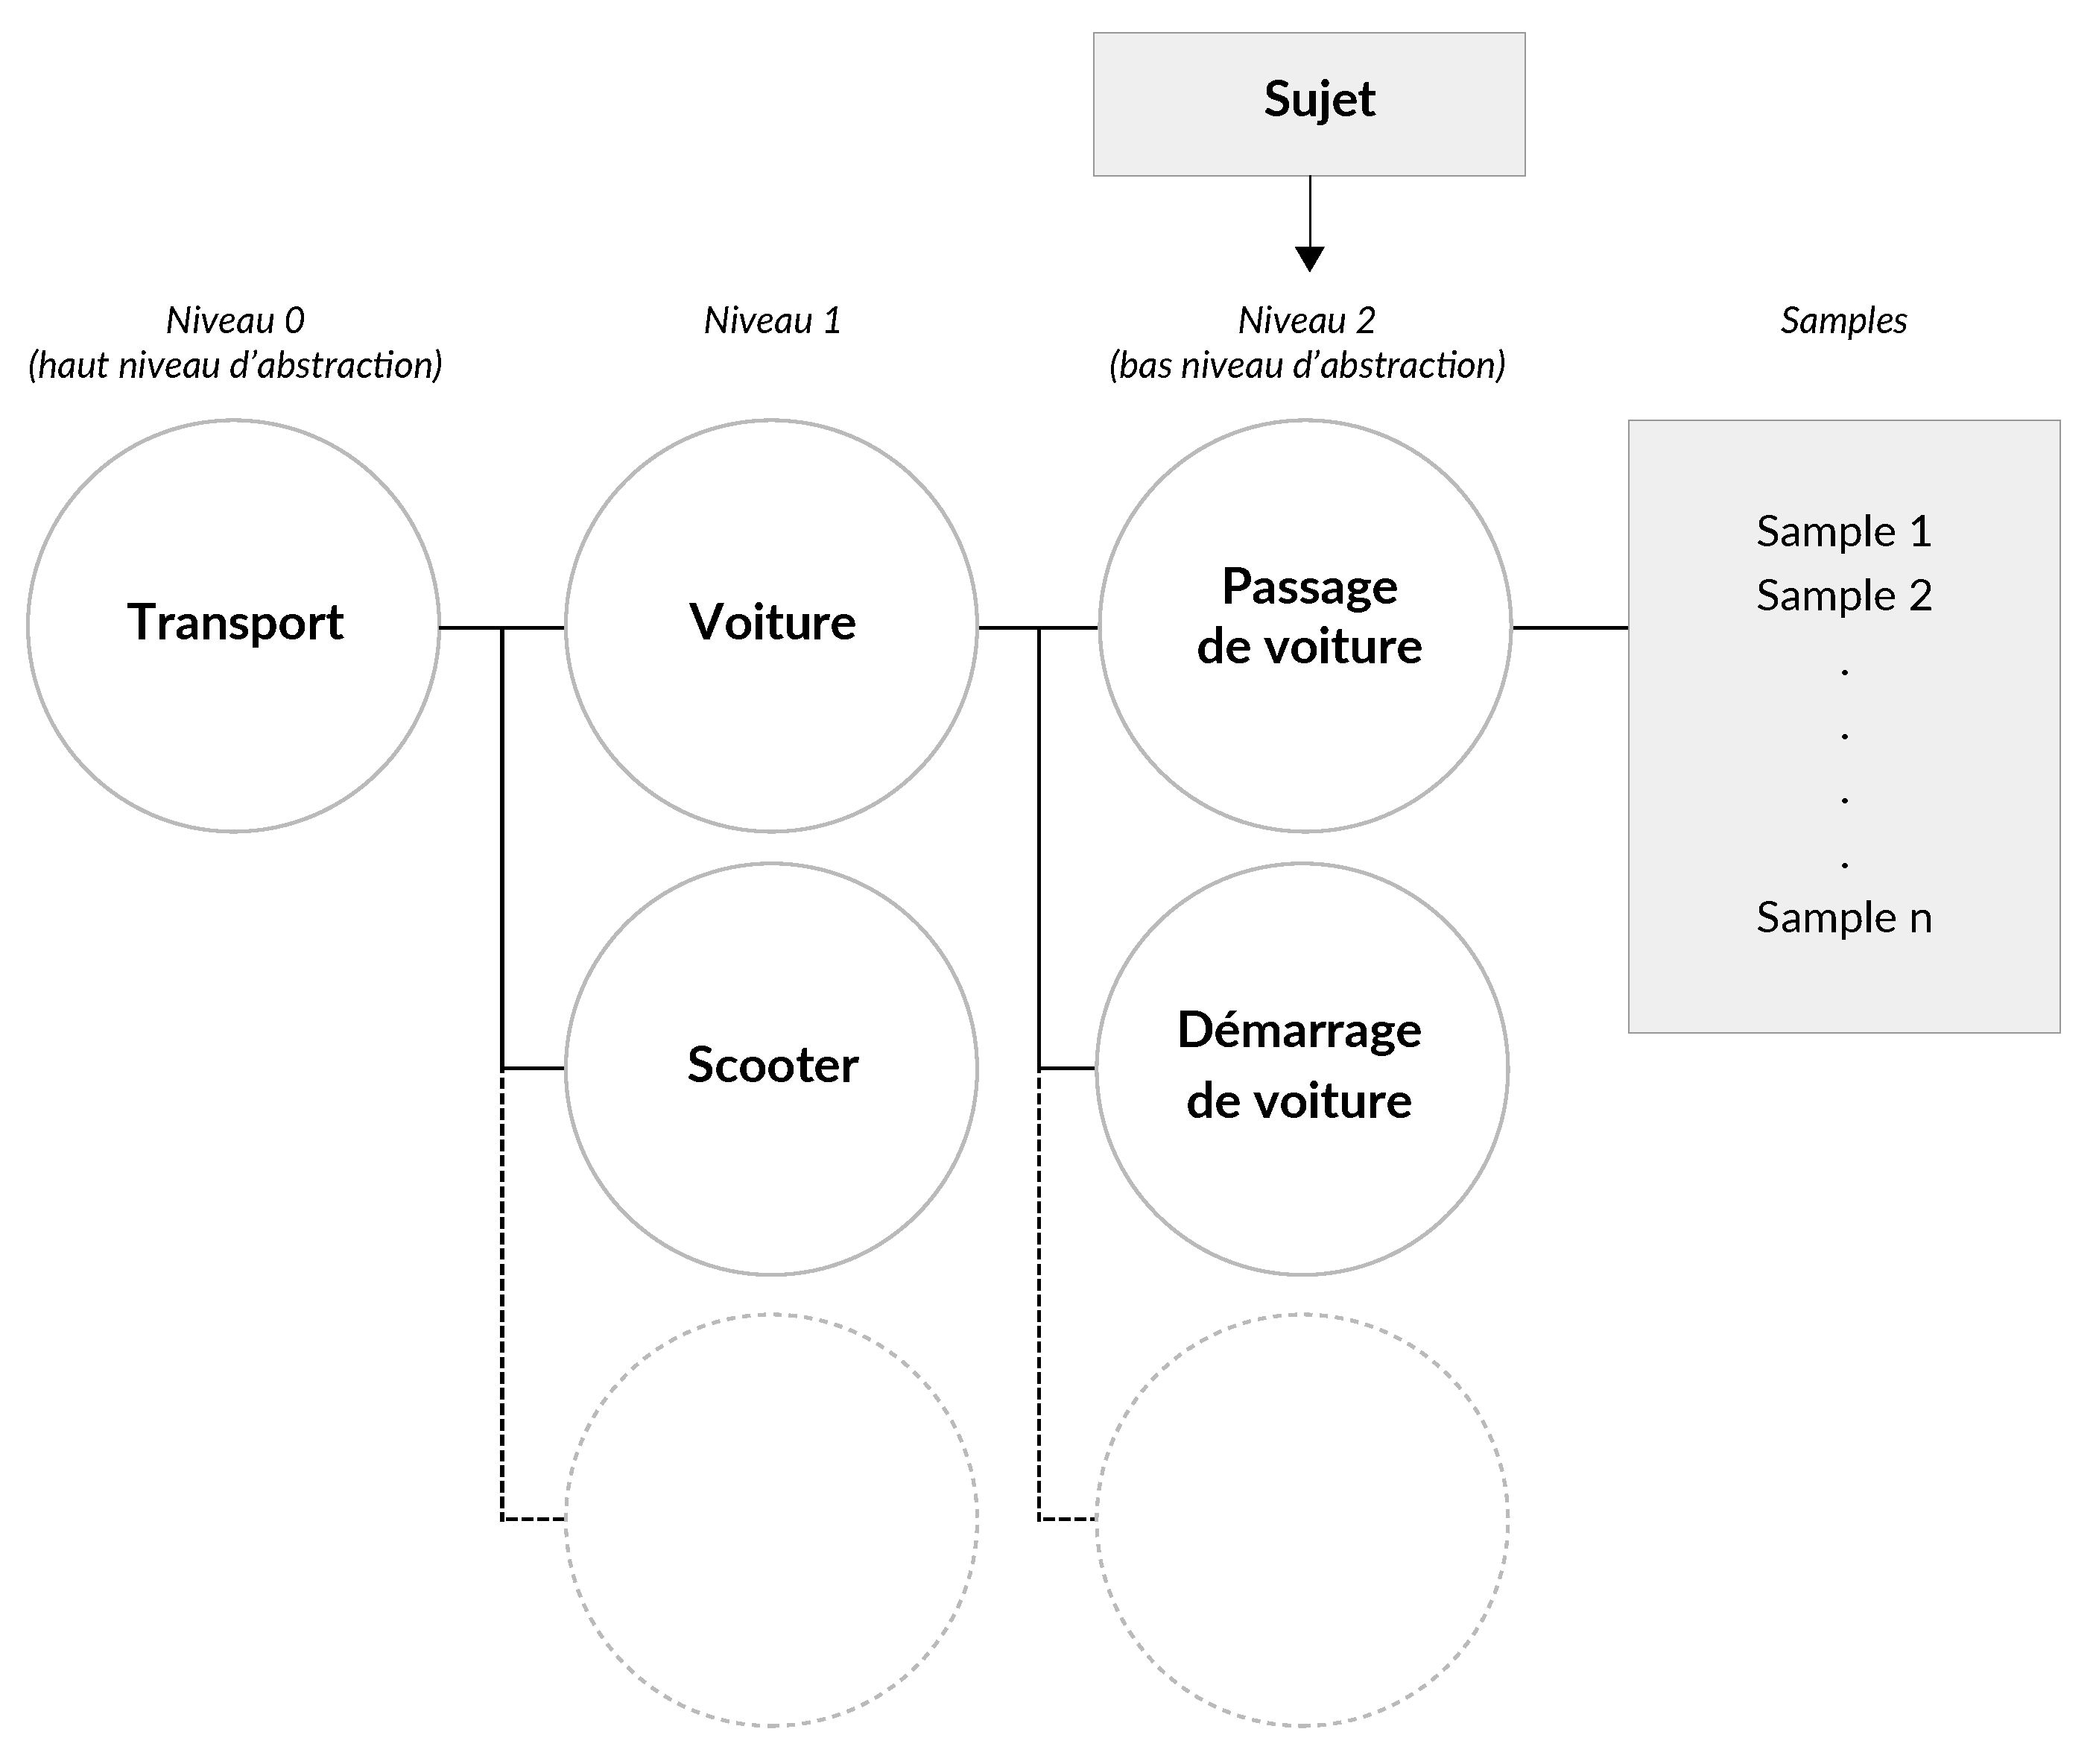
\includegraphics[width=.8\linewidth]{gfx/ch_4/3}
       \caption{Organisation hiérarchique de la banque de sons isolés utilisée pour la simulation}\label{fig:orgDb}
\end{figure}

\subsubsection{Paramètres}
\label{sec:ch4_modelParam}

En suivant la terminologie ci-devant introduite, une scène sonore est vue comme une somme de pistes. Chaque piste est une séquence temporelle, dont la structure dépend d'une série de paramètres (\cf~figure~\ref{fig:modelSequence}). Le modèle ne propose pas d’interagir avec un sample en particulier, mais toujours avec une séquence de samples.

Nous isolons trois attributs permettant de contrôler une piste:

\begin{itemize}
\item \emph{niveau}: la moyenne/variance des niveaux des samples;
\item \emph{espacement}: la moyenne/variance des espacements inter-\emph{onsets} entre les samples;
\item \emph{durée}: le début et la fin de la piste.
\end{itemize}

Le modèle fait une distinction explicite entre la gestion des pistes d'événements, et la gestion des pistes de textures. En effet, la notion de texture ne peut se comprendre que pour un son continu. Une piste de texture est donc composée de samples concaténés les uns aux autres, sans espacement (\cf~figure~\ref{fig:modelSequence}). 

Pour qu'une piste de texture soit ``\,plausible\,'', \ie~qu'on ne détecte pas de discontinuité flagrante, elle doit être une séquence composée de samples provenant de la même source, et obtenus avec un matériel (et des réglages) identique(s).

\begin{figure}[t]
        \graphicspath{{gfx/ch_4/}}
        \myfloatalign
        \def\svgwidth{\linewidth}
        \input{gfx/ch_4/controlParameters2.pdf_tex}
       \caption{TODO}\label{fig:modelSequence}
\end{figure}

\subsubsection{Formalisation du modèle}
 \label{sec:ch4_modelForm}
 
 Tout au long de nos travaux, nous avons utilisé plusieurs modèles, ainsi que différents paramètres, afin de simuler des scènes sonores. Nous formalisons, dans cette partie, une version générale du modèle proposé. Les diverses modifications appliquées au modèle, en fonction de son utilisation, sont indiquées dans les sections~\ref{sec:ch4_modAnaSo} et~\ref{sec:ch4_modAnaAuto}.
 
La formalisation présentée vaut uniquement pour les classes d'événements sonores. Nous décrivons par la suite les diverses contraintes qui s'appliquent pour une classe de textures.
 
En considérant $s$, une scène composée de $z$ classes de sons, le modèle de $s$ se définit comme suit:
 
 \begin{equation}
 s(n)=\sum_{i=1}^{z}p_i(n)
 \end{equation}

avec $n$ un indice temporel discret, et $p_i$ la piste correspondant à la classe $c_i$. La classe $c_i$ est composée de $\vert c_i\vert$ samples $c_{i,m}$, $1<m<\vert c_i\vert$. 

Une piste $p_i$ est définie comme une séquence de $n_i$ samples d'événements $e^k_i(n)$ ($k=(1,2,\ldots,n_i)$), choisis aléatoirement parmi les $\vert c_i\vert$ samples de la classe $c_i$. Considérant $\mathcal{U}(x,y)$, une distribution uniforme d'entiers allant de $x$ à $y$ ($x<y$), on a alors:

 \begin{equation}
 e^k_i=c_{i,\mathcal{U}(1,\vert c_i \vert)}
 \end{equation}

 Pour chaque piste $p_i$, un facteur d'amplitude est tiré aléatoirement à partir d'une distribution normale de moyenne $\mu^a_i$ et de variance $\sigma^a_i$. De même, les espacements inter-\emph{onsets} sont tirés d'une distribution normale de moyenne $\mu^t_i$ et de variance $\sigma^t_i$. Les indices temporels de début et de fin de chaque piste sont notés $u_i$ et $v_i$ respectivement. Formellement, une piste $p_i$ se définit comme suit:
 
\begin{equation}
\label{eq:ch4_eq1}
p_{i}(n)= \sum_{j=1}^{n_i} \mathcal{N}(\mu^a_{i},\sigma^a_{i})c_{i, \mathcal{U} (1, |c_i|)}(n-n^j_i)
\end{equation}
\begin{equation}
\label{eq:ch4_eq2}
n_i^j=n_i^{j-1} + \mathcal{N}({\mu^t_{i},\sigma^t_{i}})
\end{equation}

où $n_i^0=u_i$ par convention. Le signal d'une piste est défini de telle sorte que $p_i(n)=0$ si $n>v_i$. Les paramètres du modèle sont, $\mu^a_i$,  $\sigma^a_i$,   $\mu^t_i$,  $\sigma^t_i$, $u_i$ et $v_i$, et doivent être réglés pour chaque piste $p_i$. La figure~\ref{fig:modelSequence} offre une illustration de l'action des paramètres introduits.


Pour les textures, deux distinctions sont à observer avec le modèle défini précédemment: 

\begin{enumerate}
\item l'amplitude du signal ($\mu^a_i$,  $\sigma^a_i$) n'est tirée qu'une seule fois, et la valeur est appliquée à tous les samples;
\item afin d'éviter toute sensation de discontinuité, deux samples de texture sont concaténés en considérant un recouvrement fixé, sur lequel est appliqué un fondu enchaîné (\emph{cross-fade}) à valeur d'énergie constante entre les samples, afin de donner l'illusion de continuité.
\end{enumerate}

\gl{TODO: à revoir avec mathieu et mathias}

\section{Du modèle à la simulation: l'analyse sensorielle}
\label{sec:ch4_modAnaSo}

Dans cette section nous présentons une version du modèle précédemment introduit, afin qu'il puisse servir de base à un outils de simulation, nommé \emph{SimScene}, utilisable dans le cadre de l'analyse sensorielle des scènes sonores.

Nous commençons par présenter différents outils existant, permettant de simuler des environnements sonores. Nous proposons, par la suite, un protocole expérimental, décrivant le cadre applicatif des épreuves perceptives basées sur la simulation. Enfin, nous relions ce protocole au modèle de scènes sonores (\cf~Section~\ref{sec:ch4_modelParam}), et présentons les fonctionnalités de l'outil \emph{SimScene}.

\subsection{Simulation et analyse sensorielle}

Plusieurs outils de simulation de scènes sonores ont déjà été proposés \citep{misra2006new,misra2007musical,valle2009framework,finney2010soundscape,schirosa2010system}. Ils ont souvent pour but de générer automatiquement l'ambiance sonore d'un environnement virtuel. \citep{valle2009framework,finney2010soundscape}. Ils peuvent être vus comme des systèmes semi-autonomes: la simulation pouvant être contrôlée par un utilisateur, mais dépendant aussi, soit d'un environnement visuel à illustrer, soit d'un environnement sonore à reproduire. D'autre outils, entièrement contrôlés par un utilisateur, servent, eux, d'aide à la composition \citep{misra2006new,misra2007musical}. Ces systèmes s'éloignent tous sensiblement du cadre expérimental de l'analyse sensorielle.

A notre connaissance, seuls Bruce~\al \citep{bruce2009development,bruce2014effects} se sont servis de la simulation afin d'étudier la perception des paysages sonores. Ils proposent un système permettant au sujet d'agir sur un environnement en ajoutant ou supprimant des sources sonores spécifiques. Celui-ci peut par ailleurs modifier le niveau sonore des sources, et leurs positions spatiales.

A l'aide de cet outil, les auteurs demandent à leurs sujets de manipuler des sources, afin de recréer un environnement urbain. Les résultats montrent que l'inclusion ou l'exclusion des sources dépend plus de considérations sociales/sémantiques, que des caractéristiques physiques des sources. Ils soulignent néanmoins que le manque d'enregistrements disponibles limite l'analyse. Ils suggèrent de regrouper les enregistrements similaires en ``\,groupes sémantiques\,'' afin de faciliter l'analyse. \\

\gl{TODO G1: compléter Bruce~\al, cf wac} \\
\gl{TODO G2: \citep{davies2014soundscape} montre que, lorsqu'on demande à des participants de simuler un paysage sonore, les simulations font références à ce que ces derniers s'imaginent être un environnement typique, sans tenir compte de leur propre préférence pour des sons particuliers.}

\subsection{Protocole expérimental basé sur la simulation}

\subsubsection{Organisation des sons isolées}
\label{sec:ch4_dbEventTexture}

L'objectif de l'expérimentation est de permettre à un sujet de simuler un environnement sonore cible, à partir de sons isolés. La banque de sons suit l'organisation décrite à la section~\ref{sec:ch4_collecSons}. Les éléments sont regroupés en classes hiérarchisées, afin de former une taxonomie. Plus le niveau d'abstraction de la classe est élevé, plus la variabilité des enregistrements appartenant à la classe est importante (\cf~Figure~\ref{fig:orgDb}).
 
Nous conservons la distinction observée entre les événements et les textures, en créant deux taxonomies (\ie~deux banques de sons) séparées.

\subsubsection{Sélection des sons isolées}

L'objectif de la simulation est d'obtenir une image sonore de la représentation mentale que ce fait un sujet d'un environnement donné. Afin que cette image soit la plus ``\,juste\,'' possible, il faut que le protocole limite les biais pouvant influer sur les choix du sujet.

Un de ces biais intervient dans le processus de sélection. La grande majorité des outils permettant de parcourir une banque de données propose une recherche textuelle sur la base de mots clefs. L’efficacité de ce principe repose avant tout sur la structure typologique, et la nomenclature de la base de données. Dans le cadre d'une expérience sensorielle visant à objectiver une représentation interne d'un sujet, cette approche pose trois problèmes majeurs :

\begin{itemize}
\item les sons peuvent ne pas être tagués d'une manière satisfaisante. En effet, sémantiquement, un son peut être décrit de plusieurs façons. Nous pouvons en désigner la source (une portière de voiture), comme nous pouvons désigner l'action de la source (le claquement d’une portière de voiture) ou encore son environnement (le claquement d’une portière de voiture dans un garage). Concevoir un système de recherche par mots clefs efficace suppose une description précise de chaque son, qui plus est adaptable à la représentation que s’en fait chaque sujet, ce qui est difficilement réalisable;

\item lors d'une recherche par mots clefs, le sujet doit objectiver un nom décrivant l'objet recherché. Or cette objectivation dépend des connaissances collectives du sujet, connaissances liées à sa sphère socioculturelle, et en particulier à sa langue. L'expérience visant une diffusion internationale, cette contrainte est difficilement surmontable;

\item la description verbale du son, si elle est accessible par le sujet, peut potentiellement influencer sa sélection. Dans les faits, pour construire une scène environnementale ``\,calme\,'', le sujet sélectionne a priori les sons référencés sous le vocable \emph{parc}. Cette réalité constitue encore une difficulté.
\end{itemize}

Imposer au sujet une terminologie \gl{à travers les labels} décrivant les classes est un risque. La sélection doit s'éloigner le plus possible d'un ancrage sémantique, et s'effectuer à l'aveugle, \ie~sur la base uniquement de l'écoute. Une interface développée spécialement dans ce but est présentée à la section~\ref{sec:ch4_ssf}.

Enfin, il est important de noter que le sujet ne peut accéder qu'aux classes du niveau d'abstraction le plus bas, classes qui ne possèdent pas de sous-classes, et sont directement liées à une collection de samples.

L’organisation hiérarchique sert alors deux buts:

\begin{itemize}
\item faciliter le parcours, par les sujets, des banques de sons isolées (\cf~Section~\ref{sec:ch4_ssf});
\item faciliter le travail d'analyse de l'expérimentateur, en lui permettant d'observer la composition en terme de sources sonores des scènes, suivant différents niveaux d'abstraction.
\end{itemize}

\subsubsection{Processus de simulation}
\label{sec:ch4_processSimu}

\begin{figure}[t]
        \myfloatalign
        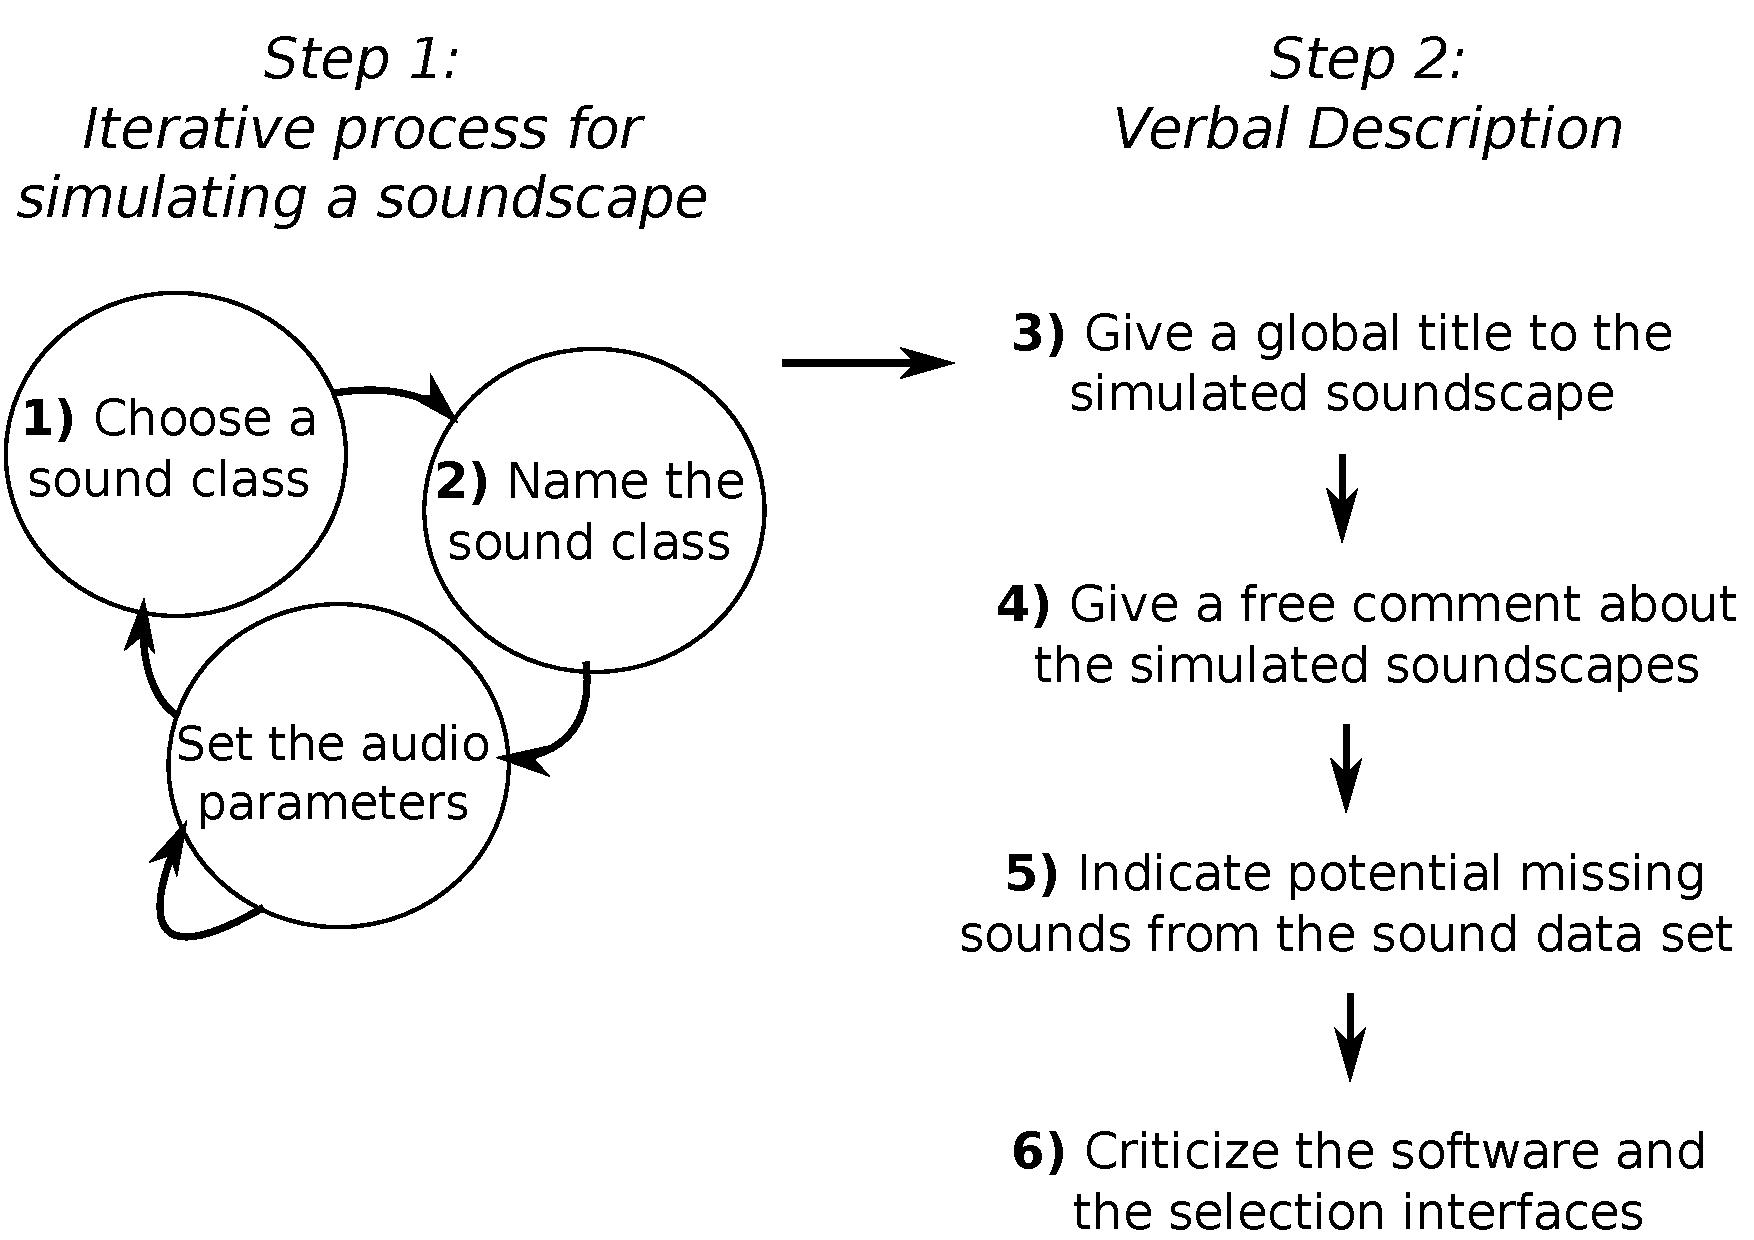
\includegraphics[width=.8\linewidth]{gfx/ch_4/4}
       \caption{Etape de processus de simulation pour l'analyse sensorielle}\label{fig:etapeSimu}
\end{figure}

Trois étapes composent le processus de simulation (\cf~Figure~\ref{fig:etapeSimu}):

\begin{itemize}
\item \emph{sélection} d'une classe de sons. Une fois une classe sélectionnée, une piste est générée; 
\item \emph{identification} de la classe de sons sélectionnée. Le sujet nomme la classe de sons qu'il a sélectionnée;
\item \emph{paramétrisation} de la piste liée à la classe de sons. Le sujet fixe les paramètres de la piste (pour plus de détails sur les paramètres proposés \cf~Section~\ref{sec:ch4_param}).
\end{itemize}

Ces étapes peuvent être répétées, et dans n'importe quel ordre, le sujet pouvant agir rétrospectivement sur les pistes déjà crées. A la fin de la simulation, et afin d'accumuler le maximum de connaissances possible sur la scène simulée, le sujet peut: 

\begin{itemize}
\item nommer l'environnement simulé;
\item fournir un commentaire libre décrivant son processus de création, ainsi que le paysage sonore qu'il a voulu illustrer.
\end{itemize}

\subsection{Paramètres de contrôle}
\label{sec:ch4_param}

Les paramètres du modèle permettent au sujet de contrôler la structure de chaque piste. Ils agissent sur tous les samples à la fois, et non sur un en particulier.

Parmi ces paramètres, on retrouve ceux introduits pour le modèle initial de scène sonore (\cf~Section~\ref{sec:ch4_modelParam} et~\ref{sec:ch4_modelForm}), à savoir:

\begin{itemize}
\item \emph{niveau sonore} ($dB$): pour chaque sample, les niveaux sont tirés aléatoirement à partir d'une distribution normale, paramétrée par le sujet en terme de moyenne et variance;
\item \emph{espacement inter-onset} (seconde): (piste d'événements seulement) comme pour les niveaux, les espacements sont tirés aléatoirement à partir d'une distribution normale, paramétrée par le sujet en terme de moyenne et variance;
\item \emph{début et fin} (seconde): le sujet fixe le début et la fin de chaque piste.
\end{itemize}

Afin de faciliter la simulation, deux paramètres supplémentaires sont proposés:

\begin{itemize}
\item \emph{fondu par événement} (seconde): (piste d'événements seulement) le sujet fixe une durée de fondu (entrée et sortie), appliquée à chaque sample d'une piste d'événements;
\item \emph{fondu global} (seconde): le sujet fixe les durées de fondus séparément, pour l'entrée et la sortie de la piste. Ces fondus s'appliquent ainsi à l'ensemble des samples de la piste.
\end{itemize}

Deux de ces paramètres ne s’appliquent que pour les pistes d'événements (\emph{fondu par événement} et \emph{espacement inter-onset}), les samples des textures étant séquencés sans espacement (\cf~Section~\ref{sec:ch4_modelParam})

\subsubsection{Données produites par le processus de simulation}

\begin{figure}[t]
        \myfloatalign
        \includegraphics[width=.8\linewidth]{gfx/ch_4/schemaXP}
       \caption{TODO}\label{fig:paradigmeSimu2}
\end{figure}

Ce protocole de simulation peut potentiellement produire un grand nombre de données. Ces dernières sont décrites à la figure~\ref{fig:paradigmeSimu2}.  Nous les résumons dans la liste suivante:

\begin{itemize}
\item données sémantiques objectives: la banque de données nous permet d'obtenir une information objective quant aux sources sonores présentes dans la scène. Les données sémantiques objectives sont les labels des classes sélectionnées;
\item données sémantiques subjectives: il s'agit des noms donnés par le sujet 1) à la scène simulée, 2) aux classes de sons sélectionnées;
\item données quantitatives issues de la partition: il s'agit de toutes les données relatives à la partition, \ie~pour chaque piste, le positionnement des samples et les paramètres (\cf~Section~\ref{sec:ch4_seqSample});
\item données quantitatives issues du signal: il s'agit d'indicateurs acoustiques extraits du signal, \eg~le niveau sonore global. Comme nous possédons les samples isolés utilisés pour la synthèse, il est possible de calculer ces descripteurs pour une classe, ou un ensemble de classes, en particulier.
\end{itemize}

Le protocole nous permet de caractériser avec précision une scène simulée, sur la base de données sémantiques, subjectives ou objectives, ainsi que quantitatives. Considérant l'ensemble des données générées, les potentiels d'analyse sont vastes.



\subsection{Interface de sélection aveugle des sons isolés}
\label{sec:ch4_ssf}

\begin{figure}[t]
        \myfloatalign
        \includegraphics[width=.8\linewidth]{gfx/ch_4/SSF}
       \caption{L'interface de sélection aveugle de l'outil de simulation \emph{Simscene}}\label{fig:ssf}
\end{figure}

Pour limiter l’influence de l’interface sur le sujet, il nous paraît nécessaire de libérer sa recherche de toute information textuelle. Nous proposons à l'utilisateur une interface graphique lui permettant d’explorer la banque de sons exclusivement à partir de l’écoute.

Visuellement, les classes du dernier niveau (les seules accessibles par le sujet) sont représentées par des cercles, et positionnées sur un plan. La disposition des cercles dans l'espace dépend de l’organisation hiérarchique de la base de données: les sous-classes appartenant à la même classe sont proches les unes des autres, et ainsi de suite jusqu'à atteindre les classes des niveaux d'abstraction élevés.

La figure~\ref{fig:ssf} présente l'interface pour la banque de données d'événements sonores. Cette organisation visuelle à été pensée afin de:

\begin{enumerate}
\item faciliter le parcours de la banque de données, les sons similaires (au sens des classes) étant proches les uns des autres. L'organisation hiérarchique se fonde, en effet, sur des principes cognitifs. Les classes ont été établies à partir de la littérature traitant des catégories de sources sonores (\cf~Section~\ref{sec:ch4_collecSons}).
\item permettre aux sujets de rapidement appréhender toute l'étendue de la banque de données, \ie~l'ensemble des sons disponibles.
\end{enumerate}

Chaque classe possède un son prototype. Ces sons ont été choisis par les expérimentateurs. Lorsqu’on ``\,clique\,'' sur un cercle, le prototype associé à la classe est joué. Le sujet parcours la banque de sons en cliquant sur les cercles.

Cette interface a fait l'objet d'une étude approfondie dont les résultats sont publiés dans \citep{lafay2016JAES}. \\

\gl{TODO: résumer les résultats JAES}

\subsection{Interface de simulation: l'outil \emph{Simscene}}
\label{sec:ch4_simscene}

\begin{figure}[t]
        \myfloatalign
        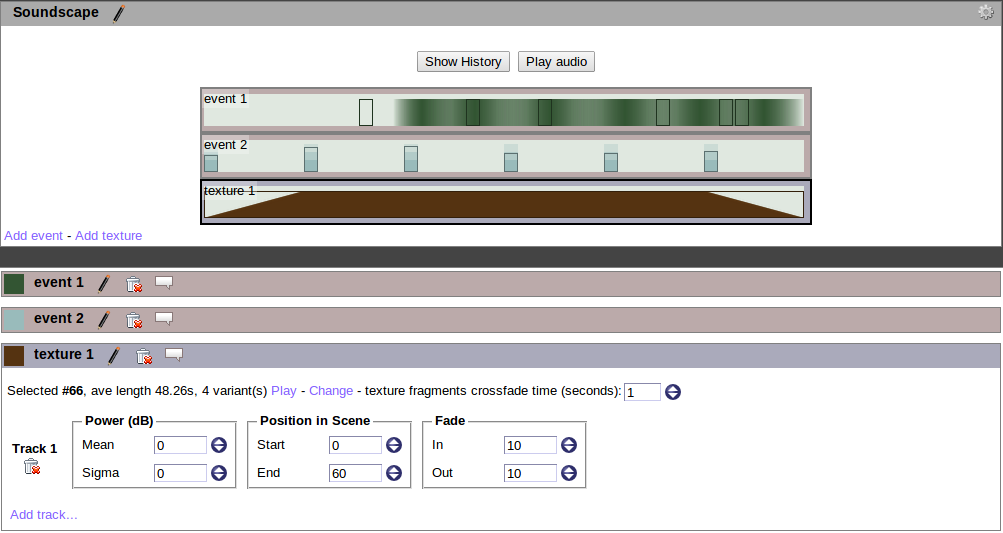
\includegraphics[width=.8\linewidth]{gfx/ch_4/simscene}
       \caption{L'outil de simulation \emph{Simscene}}\label{fig:simscene}
\end{figure}

\emph{Simscene} est un environnement de travail audio-numérique, supporté par navigateur internet, et développé dans le cadre du projet HOULE\footnote{Pour plus d’informations sur le Projet HOULE voir \url{http://houle.ircam.fr/}}. Il permet de simuler des paysages sonores à partir d'un corpus de sons. Il est prévu pour fonctionner via les navigateurs internet \emph{Chrome} et \emph{Firefox}. L'outil a été développé en javascript à l'aide de la bibliothèque \emph{angular.js}\footnote{\emph{angular.js}: \cf~\url{https://angularjs.org/}} et du standard \emph{web-audio}\footnote{\emph{web-audio}: \cf~\url{http://www.w3.org/TR/webaudio/}}. L'interface de sélection (\cf~Section~\ref{sec:ch4_ssf}) a été développée à l'aide de la bibliothèque \emph{D3.js} \citep{d32011}.

\emph{Simscene} est présenté en détail dans \citep{rossignol2015simscene}. \gl{Nous résumons ici ses fonctionnalités d'importance pour notre étude}. 

Le fonctionnement de \emph{Simscene} se rapproche de celui d'un séquenceur audio. Chaque utilisateur choisit une classe de sons via l'interface de sélection (\cf~Section~\ref{sec:ch4_ssf}). Une fois la classe de sons sélectionnée, une piste audio, liée à cette classe, est créée. L'utilisateur peut alors modifier certaines propriétés de la piste via un groupe de paramètres de contrôle propre à chacune (\cf~Section~\ref{sec:ch4_param}). Des champs de texte sont prévus afin de permettre à l'utilisateur de 1) nommer chaque piste, 2) donner un titre à la scène simulée et 3) commenter la scène simulée.

L'interface propose un rendu graphique schématisé de la scène en cours de création (\cf~Figure~\ref{fig:simscene}). La piste est représentée par une bande possédant un axe temporel. Sur cette bande, chaque sample est représenté par un rectangle. L'espacement entre les rectangles est relatif à l'espacement entre les samples. De même, la hauteur des rectangles est proportionnelle au niveau sonore des samples. Dans le cas d'une piste de texture, un unique rectangle apparaît sur toute la longueur de la piste, un son de texture ne pouvant être entrecoupé de silences. Les caractéristiques des rectangles évoluent en fonction des changements de paramètres de la piste.

L'utilisateur a la possibilité, à tout moment, d'écouter la scène simulée.

L'outil de simulation est accessible via le lien suivant: \url{http://www.irccyn.ec-nantes.fr/~lagrange/
demonstrations/simScene.html}

\section{Du modèle à la simulation: l'analyse automatique}
\label{sec:ch4_modAnaAuto}

Un ensemble dédié de fonctions Matlab, qui sont accessibles au public\footnote{https://bitbucket.org/mlagrange/simscene/downloads}.
%*****************************************
%*****************************************
%*****************************************
%*****************************************
%*****************************************
